%%!TEX TS-program = pdflatexmk
%%!TEX encoding = UTF-8 Unicode
\documentclass[11pt]{article}
\usepackage[utf8]{inputenc}

\usepackage[letterpaper,body={6.0in,9.5in},vmarginratio=1:1]{geometry}
\usepackage[small,compact]{titlesec}

\usepackage{fourier}
\usepackage[scaled=0.85]{berasans}
\usepackage[scaled=0.85]{beramono}
\usepackage{microtype}


\usepackage{xcolor}
\usepackage[colorlinks, urlcolor=darkgray, linkcolor=darkgray]{hyperref}

\usepackage{graphicx}
%\usepackage{applekeys}
% Alternate Special Keys 
\newcommand{\optkey}{\texttt{Opt}}
\newcommand{\ctlkey}{\texttt{Ctl}}
\newcommand{\cmdkey}{\texttt{Cmd}}
\newcommand{\esckey}{\texttt{Esc}}
\newcommand{\tabkey}{\texttt{Tab}}
\newcommand{\shiftkey}{\texttt{Shift}}

\newcommand{\mnu}[1]{\texttt{#1}}
\newcommand{\cmd}[1]{\texttt{#1}}
\newcommand{\To}{\,\(\to\)\,}

\pagestyle{empty}

% set | as a command character within verbatim so you can execute commands there
\usepackage{verbatim}
\makeatletter
\addto@hook\every@verbatim{\catcode`|=0}
\makeatother

% define colored items to be inserted in verbatim environments
\setlength{\fboxsep}{0pt}
\newcommand{\selmark}{\colorbox{green}{\rule[-0.5ex]{0ex}{2.1ex}\texttt{•}}}
\newcommand{\selcom}{\colorbox{green}{\rule[-0.5ex]{0ex}{2.1ex}\texttt{•‹comment›}}}
\newcommand{\selcombwra}{\colorbox{green}{\rule[-0.5ex]{0ex}{2.1ex}\texttt{•‹placement: r,R,l,L,i,I,o,O›}}}
\newcommand{\selcomrulewidth}{\colorbox{green}{\rule[-0.5ex]{0ex}{2.1ex}\texttt{•‹width›}}}
\newcommand{\selcomrulelift}{\colorbox{green}{\rule[-0.5ex]{0ex}{2.1ex}\texttt{•‹lift›}}}

% define a few items for easy use
\newcommand{\fastex}{Fas\hspace{-.15em}\TeX}
\newcommand{\TS}{\textsf{\TeX Shop}}
\newcommand{\TSVersion}{2.30}
\newcommand{\CCT}{\texttt{CommandCompletion.txt}}

\title{Quick Start Guide\\ to using\\ Command Completion with \TS}
\author{Herbert Schulz\\\small\href{mailto:herbs2@mac.com}{herbs2@mac.com}}
\date{2010/10/21}

\begin{document}
\maketitle
\thispagestyle{empty}

\section*{Introduction}

%Command Completion in \TS\ allows you quickly enter commands and environment structures into your source document. It also allows you to easily move from one argument for a command to another using built-in menu commands. This document is a simple introduction by example to using Command Completion in \TS\ while the complete documentation with lists of supplied commands and abbreviations can be found in \path{~/Library/TeXShop/CommandCompletion/Command Completion for TeXShop.pdf} where \path{~} means your HOME folder.

\LaTeX\ markup is rather wordy which is nice because it describes what it's supposed to do but a bit painful to write. Command Completion allows you to insert complete environments and commands with a few keystrokes and the press of a ``trigger'' key (this is \cmd{Esc} by default but can be changed to \cmd{Tab} in \mnu{TeXShop}\To\mnu{Preferences}\To\mnu{Source}\To\mnu{Command Completion Triggered By:}).

Commands that have arguments usually have a Mark (\texttt{•}) inserted for each argument. You move to the next argument by using the \mnu{Source}\To\mnu{Completion}\To\mnu{Marks}\To\mnu{Next Mark} command (\cmd{Ctl-Cmd-F} [or \cmd{Opt-trigger}]). This also selects the Mark so typing automatically removes the Mark and substitutes the typed information. See the complete documentation, with lists of commands/abbreviations supplied with \TS\ out of the box, in the \path{~/Library/TeXShop/CommandCompletion/} folder for much more information.

\section*{Usage}

Many commands and environments can be easily completed either by using the start of the command or a set of abbreviations to the commands and environments. The following are examples of just a few to get you started.

While the list of abbreviations is fairly extensive just learn a few that you need all the time and slowly pick up others as you need them. Also just press the trigger key multiple times to get the same commands and environments with differing numbers of options, etc.

\subsection*{Command Completion}

%On a new line type \verb|\newc| and then press \esckey\ to get:
%\begin{verbatim}
%\newcommand{|selmark}{•}
%\end{verbatim}
%while successive presses of \esckey\ give 
%\begin{verbatim}
%\newcommand{|selmark}[•]{•}
%\end{verbatim}
%and finally
%\begin{verbatim}
%\newcommand{|selmark}[•][•]{•}
%\end{verbatim}
%all with the first ``Mark'' (•) selected.
%
%You need only start to type the new command's name to replace the selected \selmark. Then select the next mark by using the \mnu{Source}\To\mnu{Completion}\To\mnu{Marks}\To\mnu{Next Mark} (\cmd{\ctlkey-\cmdkey-F} or, alternatively, \cmd{Opt-Esc} if you are using \TS\ 2.36) menu item and enter the next argument, etc. 

You can complete many commands by starting to type them and pressing the trigger key. Variations on the commands with differing numbers of optional arguments are generated by additional presses of the trigger. One example: typing \verb|\sec| on a new line and then the trigger key produces
\begin{verbatim}
\section{|selmark}
\end{verbatim}
while a second press of the trigger gives
\begin{verbatim}
\section*{|selmark}
\end{verbatim}
the *-variant of the command and a final press of the trigger gives
\begin{verbatim}
\section[|selmark]{•}
\end{verbatim}
with the optional argument.

\subsection*{Abbreviations}

%In addition to command completion there also exist many abbreviations for commands. The principal difference is that an abbreviation is a mnemonic, a short name, rather than the start of a command name. There are many abbreviations for different environments; all of them start with a `\texttt{b}'.
%
%For example typing \verb|benu| and then \esckey\ at the beginning of a line will produce the complete enumerated list environment:
%\begin{verbatim}
%\begin{enumerate}
%\item
%|selmark
%\end{enumerate}•
%\end{verbatim}
%as you might expect; the final Mark is there so it is easy to skip to the end of the environment using the \mnu{Next Mark} menu item. You can add an additional item to the list by typing \verb|ite| and press \esckey\ at the start of a new line to get and additonal
%\begin{verbatim}
%\item
%|selmark
%\end{verbatim}
%inserted at that spot. Additional handy environment abbreviations are \verb|bite|, \verb|bali|, \verb|bfig|, \verb|btabl| and \verb|btab| for the \cmd{itemize}, \cmd{align}, \cmd{figure}, \cmd{table} and \cmd{tabular} environments respectively; see the full list in the documentation.
%
%Sectioning and font variation commands also have abbreviations. Typing \verb|sec| and pressing \esckey\ on a new line produces
%\begin{verbatim}
%\section{|selmark}
%\end{verbatim}
%while additional presses of \esckey\ give the variations
%\begin{verbatim}
%\section*{|selmark}
%\end{verbatim}
%and
%\begin{verbatim}
%\section[|selmark]{•}
%\end{verbatim}
%in turn. Additional sectioning abbreviations are \verb|ssec|, \verb|sssec|, \verb|par| and \verb|spar| for \cmd{sub-section}, \cmd{sub-sub-section}, \cmd{paragraph} and \cmd{sub-paragraph} respectively.
%
%The abbreviations for font changing commands can come in-line with text so you should use them with a leading \verb|\|; \verb|\tt|, \verb|\sf|, \verb|\sc|, \verb|\em|, \verb|\bf| followed by \esckey, give \verb"\texttt{"\selmark\verb"}", \verb"\textsf{"\selmark\verb"}", \verb"\textsc{"\selmark\verb"}", \verb"\emph{"\selmark\verb"}" and \verb"\textbf{"\selmark\verb"}" respectively.

Besides completions for partial command insertions there are also many abbreviations. These are short mnemonics for complete substitutions. 

All abbreviations for environments start with a `\texttt{b}'. To generate a complete \cmd{itemize} environment place \verb|\bite| on a line by itself and press the trigger key to get
\begin{verbatim}
\begin{itemize}
\item
|selmark
\end{itemize}•
\end{verbatim}
with an extra Mark at the end so you can easily jump to the end of the environment. Additional items can be generated by typing \verb|\it| and the trigger to get
\begin{verbatim}
\item
|selmark
\end{verbatim}
ready for entry of text.

In addition to the \verb|\section| command lower level sectioning commands have abbreviations. Sub-sections can be generated by typing \verb|\ssec| and the trigger to get
\begin{verbatim}
\subsection{|selmark}
\end{verbatim}
with subsequent presses of the trigger key giving the *-variant and finally the variant with the optional argument.

As a final example \verb|\tt| and the trigger gives the \verb|\texttt{|\selmark\verb|}| command and a second press of the trigger gives the declaration \verb|\ttfamily| with similar results for other font changing commands.

\subsection*{Comments}

It is easy to remember the arguments for commands that are used fairly often but forget them for those rarely used; these are the perfect candidates for comments. An example is the order of the arguments for the \verb|\rule| command; type \verb|\rul| and the trigger key to get
\begin{verbatim}
\rule{|selcomrulewidth}{•‹height›}
\end{verbatim}
and an additional press of the trigger key gives
\begin{verbatim}
\rule[|selcomrulelift]{•‹width›}{•‹height›}
\end{verbatim}
the version with the optional argument. Another example is the \texttt{wrapfigure} environment, from the \texttt{wrapfig} package, which has multiple versions with differing numbers and positions of optional arguments. To see the variations with the comments type \verb|\bwr| on an empty line and press the trigger key to get:
\begin{verbatim}
\begin{wrapfigure}{|selcombwra}{•‹width›}
•
\end{wrapfigure}•
\end{verbatim}
with the versions with optional arguments on succeeding presses of the trigger key.

%\subsection*{Other Environments}
%
%Environments that aren't built into the \CCT\ file can always be added if you use them a lot but there is an alternative for occasional use. Built into the completion algorithm is a way to complete environments. First press \verb|\b| and \esckey\ to get \verb|\begin{|, enter the environment name and the closing \texttt{\}} and then \esckey\ again; the closing \verb|\end{}| with the corresponding environment name will be generated on a separate line.
%
%\section*{Abbreviations in \CCT}
%
%This section contains a, hopefully, complete list of the abbreviations supplied in \CCT. The list has been broken up into Environments, Commands \& Declarations and Greek Letters. If you supply a certain beginning abbreviation the search will start at the first match to what you supply and succeeding presses of \esckey\ will go down the list until there is no longer a match; e.g. if you type \texttt{be} succeeding presses of \esckey\ will match \texttt{benu}, \texttt{benuo}, \texttt{bequ}, \texttt{bequs}, \texttt{beqn} and \texttt{beqns} before returning to the original \texttt{be}. Adding more letters to the abbreviation may get you to the desired completion with fewer presses of \esckey. In reality some of the Commands \& Declarations are scattered between the Environments in the \CCT\ file so there might be additional items at times. The tables don't include standard completions or the `\verb"\"' versions of the abbreviations.
%
%\textbf{NOTE: The list may be a bit intimidating. There is no need to ``memorize'' all of these abbreviations; learn the minimum number as you need them. In addition variations on a given abbreviation are obtained by successive pressings of \esckey; e.g., see Figure \ref{fig:sec}.}
%\begin{figure}\centering
%\makebox[\textwidth]{
%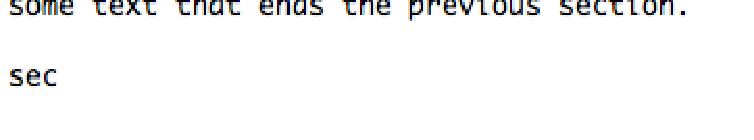
\includegraphics[width=3in]{figs/startsec}
%\hfill
\includegraphics[width=3in]{figs/sec}}
%\makebox[\textwidth]{
%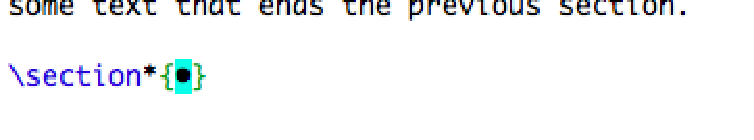
\includegraphics[width=3in]{figs/secs}
%\hfill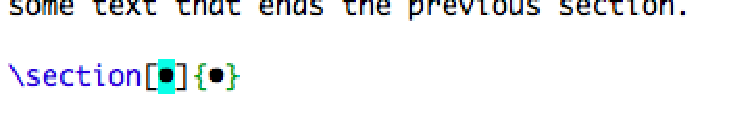
\includegraphics[width=3in]{figs/seco}}
%\caption{Initially entered \texttt{sec} and successive pressings of \esckey\ from initial to last result before returning to the beginning. Corresponds to the sequence \texttt{initial}\(\to\)\texttt{sec}\(\to\)\texttt{secs}\(\to\)\texttt{seco}.}
%\label{fig:sec}
%\end{figure}
%
%\subsection*{Environment Abbreviations}
%
%Table (\ref{tbl:environments}) on page \pageref{tbl:environments} contains a list of abbreviations for different environments supplied in \CCT. Multiple vertically adjacent Environments with the same name correspond to variations in number and distribution of possible optional arguments or \texttt{*}-variants. There can also be more than one abbreviation for the same environment.
%
%\subsection*{Commands \& Declarations}
%
%As with Environments there are lots of variations with options and \texttt{*}-variants as well as multiple abbreviations corresponding to the same command. See Table (\ref{tbl:commands}) on page \pageref{tbl:commands}.
%
%\subsection*{Greek Letters}
%
%The Greek Letter abbreviations appear in Table (\ref{tbl:greek}) on page \pageref{tbl:greek}. The in-line equation, i.e., `\texttt{d}', versions of the letters are not shown.
%
%\section*{Making Additions to \CCT}
%
%If you are adding items to the \CCT\ there are a few things you should know about its structure:
%\begin{itemize}
%\item
%Each environment has three entries: a completion that removes the leading \verb|\begin|, i.e., it starts with a leading `\texttt{\{}' and the environment name; two abbreviations that have an abbreviation name without a backslash (\verb|\|) and the same abbreviation with the backslash. Commands may have more forms; the full command as well as abbreviation(s) all with and without a leading \verb|\|.
%\item
%You should add all the variations with slightly different endings for the abbreviations. I use an `\texttt{o}' at the end of an abbreviation if that variation has an optional argument, `\texttt{oo}' for two optional arguments, `\texttt{s}' for \texttt{s}tarred forms of commands, etc.
%\item
%The order of similar items in the file \emph{does} make a dramatic difference in the order in which items are found; items placed \emph{later} will be found \emph{earlier} (the file is searched backwards). E.g., the order of items obtained when you press \verb|\b| and then \esckey\ depends purely on the order of matches in the \CCT\ file.
%\item
%For maximum convenience place a Mark\footnote{Using \texttt{Insert Mark} (\cmdkey-8) from the \texttt{Source}\(\to\)\texttt{Completion}\(\to\)\texttt{Marks} menu.} within each argument of commands. Surround the very first argument with two \verb|#INS#| commands so it comes out selected. If you want to have a comment in any arguments insert a Comment Skeleton\footnote{Using \texttt{Insert Comment} (\ctlkey-\cmdkey-8) from the \texttt{Source}\(\to\)\texttt{Completion}\(\to\)\texttt{Marks} menu.}  and fill it in.
%\end{itemize}
%I'd suggest that you take a look in the \CCT\ file for examples.
%
%\section*{Bugs}
%
%The \CCT\ file is usually searched backward from the last item but, on rare occasions, the search direction seems to switch so you don't get matches in the order you expect. You can usually force the search to go back to the ``correct'' direction by pressing \verb+---+ and then \esckey\ three times and then remove the \verb+---+. If that doesn't correct the direction you can use \shiftkey\,-\,\esckey\ to search in the ``other'' direction.
%
%\section*{What's Missing}
%
%I'd love to be able to have the completions preserve indentation but that is not in the books for now.
%
%Any other suggestions are welcome and will be considered for inclusion in later iterations of the Command Completion code.
%
%\vspace{5pt plus 2pt minus 1pt}\noindent
%Try it\dots\ I hope you like it.
%
%%\vspace{5pt plus 2pt minus 1pt}\noindent
%%Good Luck,\\
%%Herb Schulz\\
%%(\href{mailto:herbs2@mac.com}{herbs2@mac.com})
%
%\begin{table}
%\small
%\centering
%\begin{tabular}{llll}
%\textbf{Abbreviation} & \textbf{Environment} & \textbf{Abbreviation} & \textbf{Environment} \\
%\cmidrule[0.5pt](lr){1-1} \cmidrule[0.5pt](lr){2-2} \cmidrule[0.5pt](lr){3-3} \cmidrule[0.5pt](lr){4-4}
%barr      & array       & blett   & letter \\
%babs      & abstract    & blist   & list \\
%bali      & align       & bminp   & minipage \\
%balis     & align*      & bminpo  & minipage \\
%baliat    & alignat     & bmult   & multline \\
%baliats   & alignat*    & bmults  & multline* \\
%balied    & aligned     & bpict   & picture \\
%baliedat  & alignedat   & bpmat   & pmatrix \\
%baliedato & alignedat   & bquot   & quotation \\
%bapp      & appendix    & bquo    & quote \\
%bbmat     & bmatrix     & bsplit  & split \\
%bcase     & cases       & bsubeq  & subequations \\
%bcent     & center      & btab    & tabular \\
%bcenum    & compactenum & btabs   & tabular* \\
%bcenumo   & compactenum & btabx   & tabularx \\
%bcitem    & compactitem & btabl   & table \\
%bcitemo   & compactitem & btablo  & table \\
%bdes      & description & btabls  & table* \\
%benu      & enumerate   & btablso & table* \\
%benuo     & enumerate   & btbl    & table \\
%bequ      & equation    & btblo   & table \\
%bequs     & equation*   & btbls   & table* \\
%beqn      & eqnarray    & btblso  & table* \\
%beqns     & eqnarray*   & btabb   & tabbing \\
%bfig      & figure      & bbib    & thebibliography \\
%bfigo     & figure      & bindex  & theindex \\
%bframe    & frame       & btheo   & theorem \\
%bframeo   & frame       & btitpg  & titlepage \\
%bflalig   & flalign     & btrivl  & trivlist \\
%bflaligs  & flalign*    & bvarw   & varwidth \\
%bfll      & flushleft   & bverb   & verbatim \\
%bflr      & flushright  & bvers   & verse \\
%bgath     & gather      & bwrap   & wrapfigure \\
%bgaths    & gather*     & bwrapo  & wrapfigure \\
%bgathed   & gathered    & bwrapo2 & wrapfigure \\
%bgathedo  & gathered    & bwrapoo & wrapfigure \\
%bite      & itemize     &         & \\
%biteo     & itemize     &         & \\
%\end{tabular}
%\caption{Environment abbreviations supplied in \CCT.}
%\label{tbl:environments}
%\end{table}
%
%\begin{table}
%\centering
%\small
%\makebox[\textwidth]{%
%\begin{tabular}{llllll}
%\textbf{Abbreviation} & \textbf{Command} & \textbf{Abbreviation} & \textbf{Command} & \textbf{Abbreviation} & \textbf{Command} \\
%\cmidrule[0.5pt](lr){1-1} \cmidrule[0.5pt](lr){2-2} \cmidrule[0.5pt](lr){3-3} \cmidrule[0.5pt](lr){4-4} \cmidrule[0.5pt](lr){5-5} \cmidrule[0.5pt](lr){6-6}
%\texttt{-{}-}    & textendash        & midr       & midrule        & renewcomo       & renewcommand \\
%\texttt{-{}-{}-} & textemdash        & mnorm      & mathnormal     & renewcomoo      & renewcommand \\
%\texttt{-{}-{}-} & textemdash w/sp   & msf        & mathsf         & rncm            & renewcommand \\
%adlen            & addtolength       & mtt        & mathtt         & rnewc           & renewcommand \\
%adcount          & addtocounter      & mit        & mathit         & rncmo           & renewcommand \\
%bf               & textbf            & midr       & midrule        & rnewcoo         & renewcommand \\
%bfd              & bfseries          & mnorm      & mathnormal     & rncmoo          & renewcommand \\
%biblio           & bibliography      & mdd        & mdseries       & rmc             & rmfamily \\
%bibstyle         & bibliographystyle & mbox       & mbox           & rbox            & raisebox \\
%botr             & bottomrule        & makebox    & makebox        & rboxo           & raisebox \\
%bibitem          & bibitem           & mboxo      & makebox        & rboxoo          & raisebox \\
%bibitemo         & bibitem           & makebox    & makebox        & sec             & section \\
%center           & centering         & mboxoo     & makebox        & secs            & section* \\
%chap             & chapter           & mpar       & marginpar      & seco            & section \\
%cmidr            & cmidrule          & multic     & multicolumn    & ssec            & subsection \\
%cmidro           & cmidrule          & ncol       & space \& space & ssecs           & subsection* \\
%em               & emph              & ncm        & newcommand     & sseco           & subsection \\ 
%emd              & em                & newc       & newcommand     & sssec           & subsubsection \\
%foot             & footnote          & ncmo       & newcommand     & sssecs          & subsubsection* \\
%frac             & frac              & newco      & newcommand     & ssseco          & subsubsection \\
%fbox             & fbox              & ncmoo      & newcommand     & spar            & subparagraph \\
%fboxo            & framebox          & newcoo     & newcommand     & spars           & subparagraph* \\
%fboxoo           & framebox          & nct        & newcolumntype  & sparo           & subparagraph \\
%geometry         & geometry          & newct      & newcolumntype  & setl            & setlength \\
%hw               & headwidth         & newpg      & newpage        & stcount         & stepcounter \\
%hw2tw            & headw\(=\)textw   & npg        & newpage        & sf              & textsf \\
%href             & href              & nline      & newline        & sfd             & sffamily \\
%item             & item              & newlin     & newline        & sc              & textsc \\
%ito              & item              & nlen       & newlength      & scd             & scshape \\
%incg             & includegraphics   & newlen     & newlength      & sl              & textsl \\
%incgo            & includegraphics   & nenv       & newenvironment & sld             & slshape \\
%it               & textit            & newenv     & newenvironment & sqrt            & sqrt \\
%itd              & itshape           & nenvo      & newenvironment & sqrto           & sqrt \\
%latex            & LaTeX             & newenvo    & newenvironment & tt              & texttt \\
%latexs           & LaTeX w/sp        & nenvoo     & newenvironment & ttd             & ttfamily \\
%latexe           & LaTeXe            & newenvoo   & newenvironment & tw              & textwidth \\
%latexes          & LaTeXe w/sp       & pgref      & pageref        & tex             & TeX \\
%label            & label             & par        & paragraph      & texs            & TeX w/sp \\
%lbl              & label             & pars       & paragraph*     & tilde           & textasciitilde \\
%lettrine         & lettrine          & paro       & paragraph      & topr            & toprule \\
%lettrineo        & lettrine          & pgs        & pagestyle      & toc             & tableofcontents \\
%listf            & listoffigures     & parbox     & parbox         & tableofcontents & tableofcontents \\
%listt            & listoftables      & parboxo    & parbox         & tpgs            & thispagestyle \\
%rule             & rule              & parboxoo   & parbox         & thispagestyle   & thispagestyle \\
%ruleo            & rule              & parboxooo  & parbox         & up              & textup \\
%mbf              & mathbf            & pbox       & parbox         & upd             & upshape \\
%mrm              & mathrm            & pboxo      & parbox         & url             & url \\
%mcal             & mathcal           & pboxoo     & parbox         & usep            & usepackage \\
%msf              & mathsf            & pboxooo    & parbox         & usepo           & usepackage \\
%mtt              & mathtt            & ref        & ref            & verb            & verb \\ 
%mit              & mathit            & renewcom   & renewcommand   & verb2           & verb \\
%\end{tabular}
%}
%\caption{Commands and Declarations in \CCT.}
%\label{tbl:commands}
%\end{table}
%
%\begin{table}\small\centering
%\begin{tabular}{llll}
%\textbf{Abbreviation} & \textbf{Command} & \textbf{Abbreviation} & \textbf{Command} \\
%\cmidrule[0.5pt](lr){1-1} \cmidrule[0.5pt](lr){2-2} \cmidrule[0.5pt](lr){3-3} \cmidrule[0.5pt](lr){4-4}
%xa  & alpha      & xph  & phi \\
%xb  & beta       & xcph & Phi \\
%xch & chi        & xvph & varphi \\
%xd  & delta      & xps  & psi \\
%xcd & Delta      & xcps & Psi \\
%xe  & epsilon    & xs   & sigma \\
%xve & varepsilon & xcs  & Sigma \\
%xet & eta        & xvs  & varsigma \\
%xg  & gamma      & xz   & zeta \\
%xcg & Gamma      & xr   & rho \\
%xio & iota       & xvr  & varrho \\
%xl  & lambda     & xt   & tau \\
%xcl & Lambda     & xth  & theta \\
%xm  & mu         & xcth & Theta \\
%xn  & nu         & xvth & vartheta \\
%xo  & omega      & xu   & upsilon \\
%xco & Omega      & xcu  & Upsilon \\
%xp  & pi         & xx   & xi \\
%xcp & Pi         & xcx  & Xi \\
%xvp & varpi      &      & \\
%\end{tabular}
%\caption{Greek Letters in \CCT. The `\texttt{d}' versions are not shown.}
%\label{tbl:greek}
%\end{table}

\section*{Hey, the examples didn't work!}

%If the examples given here didn't work when you tried them chances are that you updated \TS\ from an older version which didn't contain the present version of the of the list of Command Completions.
%
%To update the list of Command Completions move the contents of the \path{~/Library/TeXShop/New/CommandCompletion/} folder to \path{~/Library/TeXShop/CommandCompletion/}, replacing the old \path{CommandCompletion.txt} file found there.

If these examples don't work you probably need to let \TS\ update the \path{~/Library/TeXShop/CommandCompletion/} folder; simply delete that folder from \path{~/Library/TeXShop/} and restart \TS.

\end{document}
